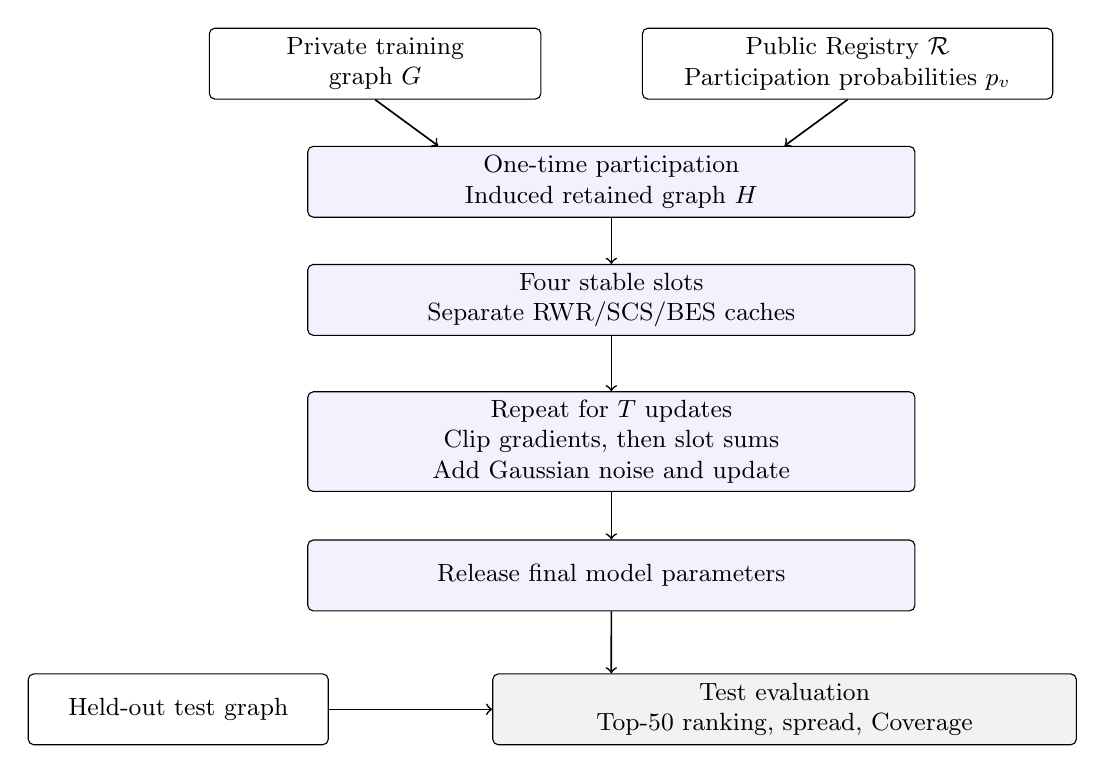
\begin{tikzpicture}[
  font=\small,
  stage/.style={draw, rounded corners=2pt, align=center, minimum height=9mm,
                inner sep=3pt, fill=blue!5},
  input/.style={stage, fill=white},
  eval/.style={stage, fill=black!5},
  flow/.style={->, semithick},
  x=1mm, y=1mm
]
\node[input, text width=40mm] (graph) at (-30,0) {Private training\\graph \(G\)};
\node[input, text width=50mm] (registry) at (30,0) {Public Registry \(\mathcal R\)\\Participation probabilities \(p_v\)};
\node[stage, text width=75mm] (retain) at (0,-15) {One-time participation\\Induced retained graph \(H\)};
\node[stage, text width=75mm] (slots) at (0,-30) {Four stable slots\\Separate RWR/SCS/BES caches};
\node[stage, text width=75mm] (updates) at (0,-48) {Repeat for \(T\) updates\\Clip gradients, then slot sums\\Add Gaussian noise and update};
\node[stage, text width=75mm] (model) at (0,-65) {Release final model parameters};
\node[input, text width=36mm] (test) at (-55,-82) {Held-out test graph};
\node[eval, text width=72mm] (evaluation) at (22,-82) {Test evaluation\\Top-50 ranking, spread, Coverage};

\draw[flow] (graph.south) -- ([xshift=-22mm]retain.north);
\draw[flow] (registry.south) -- ([xshift=22mm]retain.north);
\draw[flow] (retain) -- (slots);
\draw[flow] (slots) -- (updates);
\draw[flow] (updates) -- (model);
\draw[flow] (model.south) -- ([xshift=-22mm]evaluation.north);
\draw[flow] (test) -- (evaluation);
\end{tikzpicture}
